% This document is compiled using pdfLaTeX
% You can switch XeLaTeX/pdfLaTeX/LaTeX/LuaLaTeX in Settings

\documentclass{article}
% \usepackage[utf8]{inputenc}
\usepackage{graphicx}
\usepackage{float}
\usepackage{amssymb}
\usepackage{amsmath}
\usepackage{graphicx}
\usepackage{paralist}
\usepackage{xcolor}
\title{Assignment 5}
\author{221300079 Juntong Wang}
\date{\today}
    %\begin{figure}[H]
    %    \centering
    %    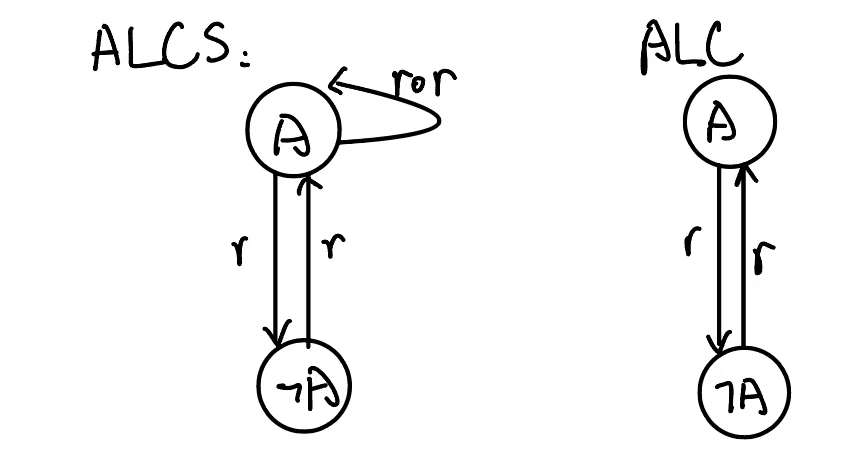
\includegraphics[width=1\textwidth]{4.png}\\
    %    \caption{Unraveling graph}
    %    \label{fig:Unraveling}
    %\end{figure}  
\newtheorem{definition}{Definition}
\setlength\parindent{0pt}

\makeatletter
\newcommand\makebig[2]{%
  \@xp\newcommand\@xp*\csname#1\endcsname{\bBigg@{#2}}%
  \@xp\newcommand\@xp*\csname#1l\endcsname{\@xp\mathopen\csname#1\endcsname}%
  \@xp\newcommand\@xp*\csname#1r\endcsname{\@xp\mathclose\csname#1\endcsname}%
}
\makeatother

\makebig{biggg} {3.0}
\makebig{Biggg} {3.5}
\makebig{bigggg}{5.0}
\makebig{Bigggg}{14.0}

\newcommand{\alc}{$\mathcal{ALC}$\xspace}
\newcommand{\el}{$\mathcal{EL}$\xspace}
\newcommand{\sig}{\textsf{sig}\xspace}
%para nao ficar o retangulo em volta dos links, apenas muda a cor dos caracteres
%para nao ficar o retangulo em volta dos links, apenas muda a cor dos caracteres

\begin{document}

	\maketitle

	\section{Question 1}
    (1) Consider the database instance $\mathcal{D}_{\textsf{PGBBW}}$ (\textsf{PGBBW} stands for \textsf{Pleasant Goat and Big Big Wolf}) below:
    
    \begin{itemize}
        \item[] \textsf{Sheep(weslie)}\quad\textsf{Sheep(slowy)}\quad\textsf{LazySheep(paddi)}
        \item[] \textsf{Sheep(tibbie)}\quad\textsf{BrownSheep(fitty)}\quad\textsf{Sheep(jonie)}
        \item[] \textsf{Wolf(wolffy)}\quad\textsf{Wolf(wolnie)}\quad\textsf{Wolf(wilie)}
        \item[] \textsf{hasFriend(weslie, slowy)}\quad\textsf{hasFriend(tibbie, jonie)}
        \item[] \textsf{hasEnemy(paddi, wolffy)}\quad\textsf{hasWife(wolffy, wolnie)}\quad\textsf{hasSon(wolnie, wilie)}
    \end{itemize}
    
    
    \noindent We query $\mathcal{D}_{\textsf{PGBBW}}$ under closed world assumption (relational database) and under open world assumption. Recall that under the closed world assumption we consider the interpretation $\mathcal{I}:=\mathcal{I}_{\mathcal{D}_{\textsf{PGBBW}}}$ defined as follows:
    
    \begin{itemize}
        \item[] $\Delta^{\mathcal{I}}=\{\textsf{weslie, slowy, paddi, tibbie, fitty, jonie, wolffy, wolnie, wilie}\}$
        \item[] $\textsf{Sheep}^{\mathcal{I}}=\{\textsf{weslie, slowy, tibbie, jonie}\}$
        \item[] $\textsf{LazySheep}^{\mathcal{I}}=\{\textsf{paddi}\}$
        \item[] $\textsf{BrownSheep}^{\mathcal{I}}=\{\textsf{fitty}\}$
        \item[] $\textsf{Wolf}^{\mathcal{I}}=\{\textsf{wolffy, wolnie, wilie}\}$
        \item[] $\textsf{hasFriend}^{\mathcal{I}}=\{(\textsf{weslie, slowy}),(\textsf{tibbie, jonie})\}$
        \item[] $\textsf{hasEnemy}^{\mathcal{I}}=\{(\textsf{paddi, wolffy})\}$
        \item[] $\textsf{hasWife}^{\mathcal{I}}=\{(\textsf{wolffy, wolnie})\}$
        \item[] $\textsf{hasSon}^{\mathcal{I}}=\{(\textsf{wolnie, wilie})\}$
    \end{itemize}
    
    
    Consider the following non-Boolean queries $F_{i}$:
    
    \begin{enumerate}
        \item $F_{1}(x)=\textsf{Wolf}(x)$ 
        \item $F_{2}(x)=\neg\textsf{Sheep}(x)$ 
        \item $F_{3}(x,y)=\textsf{hasFriend}(x,y)$ 
        \item $F_{4}(x)=\textsf{Sheep}(x)\wedge\neg\textsf{hasFriend}(x,\textsf{jonie})$
    \end{enumerate}
    
    For each $F_{i}$, give
    
    \begin{itemize}
        \item[-] for closed world assumption: \textsf{answer($F_{i}$,$\mathcal{D}_{\textsf{PGBBW}}$)};
        \item[-] for open world assumption: \textsf{certanswer($F_{i}$,$\mathcal{D}_{\textsf{PGBBW}}$)}. 
    \end{itemize}
    
    
    (2). Following (1), consider now the TBox $\mathcal{T}$ given as:
    \begin{align*}
        \textsf{LazySheep} & \sqsubseteq \textsf{Sheep}\\
        \textsf{LazySheep}\sqcap\textsf{BrownSheep} & \sqsubseteq\bot\\
        \textsf{Sheep}\sqcap\textsf{Wolf} & \sqsubseteq\bot\\
        \top & \sqsubseteq\forall\textsf{hasFriend.Sheep}\\
        \exists\textsf{hasFriend.Sheep} & \sqsubseteq\textsf{Sheep}\\
        \textsf{Sheep} & \sqsubseteq\exists\textsf{hasFriend.}\top
    \end{align*}
    Fill in the table below with the answers ``Yes'', ``No'' or ``Don't know'' to the Boolean queries.
    
    \begin{table}[ht] 
    \begin{center}
    \label{BooleanQueries}
    \scalebox{0.71}{
    \begin{tabular}{|c|c|c|c|}  
    
    \hline 
    ~Query~& ~Answer for $\mathcal{I}$~&~Certain Answer for $\mathcal{D}_{\textsf{PGBBW}}$~&~Certain Answer for $(\mathcal{T}, \mathcal{D}_{\textsf{PGBBW}})$~\\
    \hline\hline
    \textsf{LazySheep(paddi)}& Yes &  Yes& Yes \\
    \hline
    \textsf{LazySheep(fitty)}&  No  & DK & No\\
    \hline
    \textsf{Sheep(paddi)}&  No  & DK  & Yes\\
    \hline
    $\neg$\textsf{Sheep(paddi)}&   Yes & DK & No\\
    \hline
    \textsf{BrownSheep(wilie)}& No  & DK  & DK\\
    \hline
    \textsf{Wolf(fitty)}&  No &  DK & DK\\
    \hline
    \textsf{$\exists$hasFriend.$\top$(fitty)} & No  & DK & DK\\
    \hline
    \textsf{$\forall$hasFriend.$\top$(wolffy)}&  Yes  & Yes & Yes \\
    \hline
    \textsf{$\forall$hasFriend.$\exists$hasFriend.$\top$(wolnie)}& Yes   & DK  & Yes\\
    \hline
    \textsf{$\exists$hasFriend.$\forall$hasFriend.$\top$(jonie)}&  No  & DK & Yes\\
    \hline
    \end{tabular}
    }
    \end{center}

    \textbf{Here is the answer:}\\
    (1).For the closed world assumption:\\
    $Answer(F_1,D_{PGBBW})=\{wolffy, wolnie, wilie\}$\\
    $Answer(F_2,D_{PGBBW})=\{wolffy, wolnie, wilie, paddi, fitty\}$\\
    $Answer(F_3,D_{PGBBW})=\{(weslie, slowy),(tibbie, jonie)\}$\\
    $Answer(F_4,D_{PGBBW})=\{weslie, slowy, jonie\}$\\
    For the open world assumption:\\
    $CetAnswer(F_1,D_{PGBBW})=\{wolffy, wolnie, wilie\}$\\
    $CetAnswer(F_2,D_{PGBBW})=\{\emptyset\}$\\
    $CetAnswer(F_3,D_{PGBBW})=\{(weslie, slowy),(tibbie, jonie)\}$\\
    $CetAnswer(F_4,D_{PGBBW})=\{\emptyset\}$\\
    (2).The answer is in the box above:(where DK stands for Don't know)\\
    
    \end{table}
    
    \section{Question 2}
    \textbf{Computing $\mathcal{I}_{\mathcal{T},\mathcal{A}}$ in $\mathcal{EL}$}\\
    Consider the following $\mathcal{EL}$ TBox $\mathcal{T}$:
    \begin{align*}
        \textsf{Vocalist} & \sqsubseteq \exists\textsf{plays\_for.Band}\\
        \textsf{Guitarist} & \sqsubseteq \exists\textsf{plays\_for.Band}\\
        \textsf{Bassist} & \sqsubseteq \exists\textsf{plays\_for.Band}\\
        \textsf{Drummer} & \sqsubseteq \exists\textsf{plays\_for.Band}\\
        \textsf{LeadGuitarist} & \sqsubseteq\textsf{Guitarist}\\
        \textsf{RhythmGuitarist} & \sqsubseteq\textsf{Guitarist}\\
        \textsf{Band} & \sqsubseteq\exists\textsf{captained\_by.Captain}\\
        \textsf{Band} & \sqsubseteq\exists\textsf{managed\_by.Manager}\\
        \textsf{Manager} & \sqsubseteq \exists\textsf{managed\_by.Manager}
    \end{align*}

    and the following ABox $\mathcal{A}$:
    \begin{align*}
        \textsf{Captain(Monster)}\quad &\textsf{Vocalist(Ashin)}\\
        \textsf{LeadGuitarist(Monster)}\quad & \textsf{Bassist(Masa)}\\
        \textsf{RhythmGuitarist(Stone)}\quad & \textsf{Drummer(Ming)}\\
        \textsf{Band(Mayday)}\quad & \textsf{managed\_by(Mayday, Amuse)}
    \end{align*}~\\~\\~\\~\\
    \begin{itemize}
    \item[-] Compute the interpretation $\mathcal{I}_{\mathcal{T},\mathcal{A}}$ as described in the slides.
    \item[-] For $\mathcal{EL}$ concept queries, we know that $\mathcal{I}_{\mathcal{T},\mathcal{A}}$ gives the answer ``Yes'' iff $(\mathcal{T}, \mathcal{A})$ gives the certain answer ``Yes''. Check this for the following queries:
    \begin{enumerate}
    \item \textsf{$\exists$plays\_for.Band(Ashin);}
    \item \textsf{$\exists$managed\_by.Manager(Masa);}
    \item \textsf{$\exists$plays\_for.$\exists$captained\_by.Captain(Monster);}
    \item \textsf{$\exists$plays\_for.$\exists$managed\_by.Manager(Ming).}
    \end{enumerate}
    \item[-] For more complex queries, $\mathcal{I}_{\mathcal{T},\mathcal{A}}$ can give the answer ``Yes'' even if $(\mathcal{T}, \mathcal{A})$ does not give the certain answer ``Yes''. Check this for:
    \begin{enumerate}
    \item $F(x,y)=\exists z.(\textsf{plays\_for}(x,z)\wedge\textsf{plays\_for}(y,z))$.
    \item $F=\exists x.\textsf{managed\_by}(x,x)$.
    \end{enumerate}
    \end{itemize}

    \textbf{Here is the answer:}\\
    (1):The initial situation like this:
    \begin{itemize}
        \item $S(d_{Vocalist}) = \{Vocalist\}$
        \item $S(d_{Guitarist}) = \{Guitarist\}$
        \item $S(d_{Bassist}) = \{Bassist\}$
        \item $S(d_{Drummer}) = \{Drummer\}$
        \item $S(d_{LeadGuitarist}) = \{LeadGuitarist\}$
        \item $S(d_{RhythmGuitarist}) = \{RhythmGuitarist\}$
        \item $S(d_{Band}) = \{Band\}$
        \item $S(d_{Captain}) = \{Captain\}$
        \item $S(Monster) = \{Captain\}$
        \item $S(Ashin) = \{Vocalist\}$
        \item $S(Monster) = \{LeadGuitarist\}$
        \item $S(Masa) = \{Bassist\}$
        \item $S(Stone) = \{RhythmGuitarist\}$
        \item $S(Ming) = \{Drummer\}$
        \item $S(Mayday) = \{Band\}$
        \item $S(Amuse) = \{\emptyset\}$
        \item $R(managed\_by) = \{(Mayday, Amuse)\}$
        \item $R(captained\_by) = \{\emptyset\}$
        \item $R(plays\_for) = \{\emptyset\}$
    \end{itemize}
    
    Then, we use the rules in the slides(simpleR):\\
    \begin{itemize}
        \item $S(d_{LeadGuitarist}) = \{LeadGuitarist, Guitarist\}$
        \item $S(d_{RhythmGuitarist}) = \{RhythmGuitarist, Guitarist\}$
    \end{itemize}
    
    Then, we use the rules in the slides(rightR):\\
    \begin{itemize}
        \item $R(managed\_by) = \{(Mayday, Amuse), (d_{Band}, d_{Manager}), (Mayday, d_{Manager}), (d_{Manager}, d_{Manager})\}$
        \item $R(captained\_by) = \{(d_{Band}, d_{Captain}), (Mayday, d_{Captain})\}$
        \item $R(plays\_for) = \{(d_{Vocalist}, d_{Band}), (Ashin, d_{Band}), (d_{Guitarist}, d_{Band}), (Monster, d_{Band}), \\
        (Stone, d_{Band}), (d_{Bassist}, d_{Band}), (Masa, d_{Band}), (d_{Drummer}, d_{Band}), (Ming, d_{Band})\}$
    \end{itemize}
    
    So the final we have:\\
    \begin{itemize}
        \item $\Delta^{I_{T,A}} = \{d_{Vocalist}, d_{Guitarist}, d_{Bassist}, d_{Drummer}, d_{LeadGuitarist}, d_{RhythmGuitarist}, d_{Band}, \\
        d_{Captain},Monster, Ashin, Masa, Stone, Ming, Mayday, Amuse\}$
        \item $Guitarist^{I_{T,A}} = \{d_{Guitarist}, Monster, Stone\}$
        \item $Vocalist^{I_{T,A}} = \{d_{Vocalist}, Ashin\}$
        \item $Bassist^{I_{T,A}} = \{d_{Bassist}, Masa\}$
        \item $Drummer^{I_{T,A}} = \{d_{Drummer}, Ming\}$
        \item $LeadGuitarist^{I_{T,A}} = \{d_{LeadGuitarist}, Monster\}$
        \item $RhythmGuitarist^{I_{T,A}} = \{d_{RhythmGuitarist}, Stone\}$
        \item $Band^{I_{T,A}} = \{d_{Band}, Mayday\}$
        \item $Captain^{I_{T,A}} = \{d_{caption}, Monster\}$
        \item $R(managed\_by) = \{(Mayday, Amuse), (d_{Band}, d_{Manager}), (Mayday, d_{Manager}),\\
         (d_{Manager}, d_{Manager})\}$
        \item $R(captained\_by) = \{(d_{Band}, d_{Captain}), (Mayday, d_{Captain})\}$
        \item $R(plays\_for) = \{(d_{Vocalist}, d_{Band}), (Ashin, d_{Band}), (d_{Guitarist}, d_{Band}), (Monster, d_{Band}),$
            $(Stone, d_{Band}), (d_{Bassist}, d_{Band}), (Masa, d_{Band}), (d_{Drummer}, d_{Band}), (Ming, d_{Band})\}$ 
    \end{itemize}

    (2).For this question:\\
    2.1:{$\exists$plays\_for.Band(Ashin);}\\
    We look for the relation playes-for and check if have (Ashin, Band),here the answer is Yes.\\
    So the certain answer is Yes.\\

    2.2:{$\exists$managed\_by.Manager(Masa);}\\
    We look for the relation managed-by and check if have (Masa, Manager),here the answer is No.(not Yes)\\
    So the certain answer is No.(not Yes)\\

    2.3:{$\exists$plays\_for.$\exists$captained\_by.Captain(Monster);}\\
    We look for the relation playes-for and captained-by and check if have $(Monster, d_{Band}),\\
    (d_{Band}, d_{Captain})$,here the answer is Yes.\\
    So the certain answer is Yes.\\

    2.4:{$\exists$plays\_for.$\exists$managed\_by.Manager(Ming).}\\
    We look for the relation playes-for and managed-by and check if have $(Ming, d_{Band}),\\
    (d_{Band}, d_{Manager})$,here the answer is Yes.\\
    So the certain answer is Yes.\\

    (3).For this question:\\
    3.1.$F(x,y)=\exists z.(\textsf{plays\_for}(x,z)\wedge\textsf{plays\_for}(y,z))$.\\
    we could find that every relation in the plays-for, the second part always be the $d_{Band}$, so every first part could be the answer of F(x,y).\\
    So the answer is a lot which looks like in this form:$(1\ of\ 7\ first\ part, 7\ parts)$.There are 49 elements.\\
    But the certain is $(Ashin, Ashin),(Monster, Monster),(Stone, Stone),(Masa,Masa)\\
    (Ming,Ming)$.So could give Yes.\\ 
    
    3.2.$F=\exists x.\textsf{managed\_by}(x,x)$.\\
    In the rule of manager-by, we have $(d_{Manager}, d_{Manager})$ the answer is Yes.\\
    But the certain answer could not be Yes, because we don't the answer in (T,A).\\

	\section{Question 3}
    Consider the following database $\mathcal{D}$ consisting of the following tables:
    \begin{table}[ht] 
    \begin{center}
    \label{table1}
    \scalebox{1.0}{
    \begin{tabular}{|c|c|}  
    Person: & \\
    \hline 
    ID~& Name \\
    \hline
    \textsf{2101}&  \textsf{Jay\_Chou}\\
    
    \textsf{2102}&  \textsf{Jolin\_Tsai}\\
    
    \textsf{2103}&  \textsf{Stefanie\_Sun}\\
    
    \textsf{2104}&  \textsf{Ta-yu\_Lo}\\
    \hline
    \end{tabular}
    }\scalebox{1.0}{
    \begin{tabular}{|c|c|}  
    Enrollment: & \\
    \hline 
    StudentID~& Since \\
    \hline
    \textsf{2102}&  \textsf{2020}\\
    
    \textsf{2103}&  \textsf{2021}\\
    
    \textsf{2104}&  \textsf{2020}\\
    
    & \\
    \hline
    \end{tabular}
    }\scalebox{1.0}{\begin{tabular}{|c|c|} 
    Attendance: &\\
    \hline 
    StudentID~& CourseID \\
    \hline
    \textsf{2101}&  \textsf{30000160}\\
    
    \textsf{2102}&  \textsf{30000160}\\
    
    \textsf{2102}&  \textsf{30000170}\\
    
    \textsf{2103}&  \textsf{30000150}\\
    \hline
    \end{tabular}
    }\scalebox{1.0}{\begin{tabular}{|c|c|}  
    Course: &\\
    \hline 
    ID~& Title \\
    \hline
    \textsf{30000150}&  \textsf{ML}\\
    
    \textsf{30000160}&  \textsf{KRP}\\
    
    \textsf{30000170}&  \textsf{NLP}\\
    
    &  \\
    \hline
    \end{tabular}
    }
    \end{center}
    \end{table}
    \begin{itemize}
        \item[-] Define the finite first-order interpretation $\mathcal{I}_{\mathcal{D}}$ corresponding to $\mathcal{D}$. 
        \item[-] Reformulate each of the following SQL queries $Q$ into first-order queries $f_{Q}$, and identify which of them are conjunctive queries.
        \item[-] Answer $Q$ in the context of $\mathcal{D}$ and $f_{\mathcal{Q}}$ in the context of $\mathcal{I}_{\mathcal{D}}$.
        \item[]\begin{itemize}
        \item[1.] \textsf{SELECT} $\ast$ \textsf{FROM} Person
        \item[2.] \textsf{SELECT} Person.Name \textsf{FROM} Person, Attendance, Course\\
           \text{\textsf{WHERE} Person.ID} = \text{Attendance.PersonID}\\
           \text{~~~~~\textsf{AND} Course.ID} = \text{Attendance.CourseID}\\
           \text{~~~~~\textsf{AND} Course.Title} = ``\textsf{KRP}''
        \item[3.] \textsf{SELECT} Person.Name \textsf{FROM} Person, Enrollment\\
           \text{\textsf{WHERE} Person.ID} = \text{Enrollment.PersonID}\\
           \textsf{AND NOT EXISTS (}\\
           \text{~~~~~\textsf{SELECT}} $\ast$ \textsf{FROM} Attendance\\
           \text{~~~~~\textsf{WHERE}} Person.ID = Attendance.PersonID\textsf{)}
    \end{itemize}
    \end{itemize}
    \textbf{Here is the answer:}\\
    (1).The $I_D$ is as follow:\\
    \begin{itemize}
        \item $ID^{I_D}=\{2101, 2102, 2103, 2104, 30000150, 30000160, 30000170\}$
        \item $Name^{I_D}=\{Jay\_Chou, Jolin\_Tsai, Stefanie\_Sun, Ta-yu\_Lo\}$
        \item $StudentID^{I_D}=\{2101, 2102, 2103, 2104\}$
        \item $Since^{I_D}=\{2020, 2021\}$
        \item $CourseID^{I_D}=\{30000150, 30000160, 30000170\}$
        \item $Title^{I_D}=\{ML, KRP, NLP\}$
        \item $Person^{I_D}=\{(2101,Jay\_Chou),(2102,Jolin\_Tsai),(2103,Stefanie\_Sun),(2104,Ta-yu\_Lo)\}$
        \item $Enrollment^{I_D}=\{(2102,2020),(2103,2021),(2104,2020)\}$
        \item $Attendance^{I_D}=\{(2101,30000160),(2102,30000160),(2102,30000170),(2103,30000150)\}$
        \item $Course^{I_D}=\{(30000150,ML),(30000160,KRP),(30000170,NLP)\}$
    \end{itemize}
    (2).The answer of changing the under 3 sequence into $f_Q$ are as followed:\\
    1.$F(x,y) = Person(x,y)$\\
    2.$F(x) = \exists z\exists x(Person(x,y)\wedge Attendance(x,z)\wedge Course(z,KRP))$.\\
    3.$F(x) = \exists z\exists x(Person(x,y)\wedge Enrollment(x,z)\wedge \forall w \neg Attendance(x,w))$ \\
    In the following 3 $f_Q$s we could get that the 1 and 2 are conjunctive query, and the 3 has forall, so it is not the conjunctive query.

    (3).When in D context:\\
    1.$\{(2101,Jay\_Chou),(2102,Jolin\_Tsai),(2103,Stefanie\_Sun),(2104,Ta-yu\_Lo)\}$\\
    2.$\{Jay\_Chou, Jolin\_Tsai\}$\\
    3.$\{Ta-yu\_Lo\}$\\
    When in $f_Q$ context:\\
    1.$\{(2101,Jay\_Chou),(2102,Jolin\_Tsai),(2103,Stefanie\_Sun),(2104,Ta-yu\_Lo)\}$\\
    2.$\{Jay\_Chou, Jolin\_Tsai\}$\\
    3.$\{Ta-yu\_Lo\}$\\

	\section{Question 4}
    Consider the following $\mathcal{ALC}$ knowledge base $\mathcal{K}:=(\mathcal{T},\mathcal{A})$ with:
    \begin{align*}
        \mathcal{T} := & \{\textsf{$\textsf{X}\sqsubseteq Y, Y\sqsubseteq\exists r.X, X\sqsubseteq\forall r.Y, \forall r.X\sqsubseteq Y, W\equiv\neg V, \exists r.Y\sqsubseteq\neg V$}\}\\
        \mathcal{A} := & \{\text{(Jay\_Chou, Jolin\_Tsai)} : r, \text{(Jolin\_Tsai, Stefanie\_Sun)} : r, \text{(Stefanie\_Sun, Jay\_Chou)} : r,\\
        & \text{\textcolor{white}{\{}(Jolin\_Tsai, Jolin\_Tsai)} : r, \text{(Stefanie\_Sun, Stefanie\_Sun)} : r, \text{Stefanie\_Sun} : X\}
    \end{align*}
    \begin{itemize}
        \item[-] Compute the certain answers to the following conjunctive queries in the context of $\mathcal{A}$.
        \item[-] Compute the certain answers to the following conjunctive queries in the context of $\mathcal{K}$.
        \item[]\begin{itemize}
            \item[1.] $r(x, y)\wedge Y(y)$
            \item[2.] $\exists y(r(x, y)\wedge Y(y))$
            \item[3.] $\exists x,y(r(x, y)\wedge r(y, x))$
            \item[4.] $\exists z,w(r(x, y)\wedge r(y, z)\wedge r(z, x)\wedge r(z, w)\wedge W(w))$
        \end{itemize}
    \end{itemize}
    \textbf{Here is the answer:}\\
    First, with context of A:\\
    1.certain answer:$\emptyset$\\
    2.certain answer:$\emptyset$\\
    3.certain answer:$\{(Stefanie\_Sun, Stefanie\_Sun),(Jolin\_Tsai, Jolin\_Tsai)\}$,So it is $\top$\\
    4.certain answer:$\emptyset$\\

    Second, with the context K:\\
    1.certain answer:$(Jolin\_Tsai, Stefanie\_Sun),(Stefanie\_Sun, Stefanie\_Sun),\\
    (Stefanie\_Sun, Jay\_Chou)$\\
    2.certain answer:$\{Stefanie\_Sun, Jay\_Chou\}$\\
    3.certain answer:$\{(Stefanie\_Sun, Stefanie\_Sun),(Jolin\_Tsai, Jolin\_Tsai)\}$,So it is $\top$\\
    4.certain answer:$\{(Stefanie\_Sun, Stefanie\_Sun), (Jolin\_Tsai, Jolin\_Tsai),\\
     (Jay\_Chou, Jolin\_Tsai), (Jolin\_Tsai, Stefanie\_Sun),(Stefanie\_Sun, Jay_Chou)\}$\\

    \section{Question 5}
    CW5 focuses on implementing an OWL-based querying system. Your primary task involves querying the reasoner for sub-classes, equivalent classes, and instances, then storing these results in a QueryResult object. Within the Java class CW5, you are expected to implement specific methods. Please ensure you do not modify any classes other than CW5, as this is the only class you may submit. To evaluate your implementation, you can utilize the provided classes, App.java and PizzaOrderingSystemApp.java. These classes provide a user-friendly way to verify your code's correctness. You can run these classes in Eclipse (or your preferred IDE) by clicking the small white and green arrow icon when the class is open. For a more direct approach, consider using the pre-implemented unit tests to gauge your progress. Note that passing these unit tests does not guarantee a perfect score, as additional tests will be used to assess your solution more comprehensively. Upon completing the assignment, please compress your CW5.java into a zip file for submission. Good luck!
    \begin{enumerate}
    \item {\textsf{public Set$<$QueryResult$>$ performQuery (OWLClassExpression exp, Query Type type) \{...\}}}\\
    This method takes in an arbitrary expression in OWL, like ``Person and hasBirthYear value 1964'' or ``hasTopping some MeatTopping'' and queries the ontology for the following three types of knowledge:\\
    EquivalentClasses: you are asked to return all those (named) classes that are equivalent to the expression (exp), using the (already fully initialized) reasoner.\\
    Sub-classes: return all those classes that are (named) sub-classes of the expression, using the reasoner.\\
    Instances: return all those individuals that are instances of the expression, using the reasoner.\\
    Query results are stored in query result objects. These are created for example as follows:\\
    {\textsf{QueryResult qr = new QueryResult(ind, false, type);}}\\
    Note that you need to include the information whether the inference is direct or indirect. Example: Given three classes with A subclass B subclass C, then A is a direct subclass of B and B is a direct subclass of C, but A is an indirect subclass of C (through B!). In order to solve this problem, you will query the reasoner for direct and indirect sub-class separately. After creating the QueryResult, add it to the provided set.
    \item {\textsf{public Boolean isValidPizza (OWLClassExpression exp) \{...\};}}\\
    In this method, you check whether the supplied class expression exp is a valid pizza expression, i.e., whether it is inferred to be a Pizza.
    \item {\textsf{public Set$<$QueryResult$>$ filterNamedPizzas (Set$<$QueryResult$>$ results) \{...\};}}\\
    This question is similar to the one before, only that you are asked to filter from a set of results those that correspond to NamedPizza's, such as Margherita or AmericanHot.
    \item {\textsf{public Set$<$OWLClassExpression$>$ getAllSuperClassExpressions (OWLClass ce) \{...\};}}\\
    \end{enumerate}
    This question requires a bit of thinking. You are asked to query the ontology to gather all available information about the class \textsf{ce}. In order to get an idea of what ``AL'' means, you can open Prot\'eg\'e and look at the ``Classe'' tab. Clicking on a class will reveal its super-classes, equivalent-classes, as well as inherited super-classes (Anonymous Ancestors) and indirect super-classes. Unfortunately, the reasoner will not easily give you access to those. In order to get full marks for this task, it is sufficient to query for all super-classes (direct and indirect, using the reasoner), and somehow find a way to obtain the anonymous super-classes using the ontology directly (that will need a bit of thought, do not despair too quickly). A perfect solution will test, for all sub-expressions in the ontology, whether \textsf{ce} is a sub-concept of it. Attempt this only if you are really confident with the OWL API by now.


    \section{Question 6}
    The problem is too long, so here we only give out the answer of the 3 question:\\
    \begin{itemize}
        \item[-] Show that for every two $\mathcal{L}$-TBoxes $\mathcal{T}_2$, $\mathcal{T}_{1}\subseteq\mathcal{T}_{2}$, and a signature $\Sigma$ over $\mathcal{L}$, if $\mathcal{T}_{2}$ is a model $\Sigma$-conservative extension of $\mathcal{T}_{1}$, then it is a also deductive $\Sigma$-conservative extension of $\mathcal{T}_{1}$.
        \item[-] Show that there exists two $\mathcal{ALC}$-TBoxes $\mathcal{T}_2$, $\mathcal{T}_{1}\subseteq\mathcal{T}_{2}$ such that $\mathcal{T}_{2}$ is a deductive $\Sigma$-conservative extension of $\mathcal{T}_{1}$ but it is NOT a model conservative extension of $\mathcal{T}_{1}$.
        \item[-] Consider the TBox $\mathcal{P}_{1}$ consisting of the axioms \textsf{P1---P4} and \textsf{E1} and the TBox $\mathcal{Q}$ consisting of the axioms $\textsf{M1---M5}$ from Figure~$1$. Show that $\mathcal{P}_{1}\cup\mathcal{Q}$ is a deductive conservative extension of $\mathcal{Q}$.
    \end{itemize}
    \textbf{Here is the answer}\\
    (1).As the problem goes, if we need to prove it is also a $\Sigma-conservative\ extension$ of $T_1$, we need to prove like:\\
    we assume we have a $T_2$, and $T_2$ is a $\Sigma$ conservative extension of $T_1$.so if we have L-axiom $
    \alpha$ that $sig(\alpha)\subseteq\Sigma$, so for every model of $T_1$, we have $I_1 \models \alpha$. 
    So for every model of $I_1$, if $T_2$ is a $\Sigma$ conservative extension of $T_1$, there must be the model $I_2$ according to the problem that we could get
    $I_2 \models T_2$ and also $I_1|\Sigma = I_2|\Sigma$,so for $\alpha$, there is $I_2\models \alpha$.\\
    So $T_2 \models \alpha$ if $T_1\models \alpha$.\\
    Also if we suppose $T_2\models \alpha$,  akso we could find $I_2$ that $I_2\models \alpha$,and then we could get the same $I_1 \models T_1$,$I_1|\Sigma = I_2|\Sigma$.
    So $I_1 \models \alpha,T_1 \models\alpha$ .\\
    In the end, we proved that for every two $\mathcal{L}$-TBoxes $\mathcal{T}_2$, $\mathcal{T}_{1}\subseteq\mathcal{T}_{2}$, and a signature $\Sigma$ over $\mathcal{L}$, if $\mathcal{T}_{2}$ is a model $\Sigma$-conservative extension of $\mathcal{T}_{1}$, then it is a also deductive $\Sigma$-conservative extension of $\mathcal{T}_{1}$.\\
    (2)Here is a example:$T_1:\{A\sqsubseteq \exists r.B\}$,$T_2:\{A\sqsubseteq \exists r.B,B\sqsubseteq \exists r.C\}$,and $\Sigma=\{A,B,r\}$\\
    $T_2$ is a deductive $\Sigma-$conservative of $T_1$,this is easy, and $T_2$ is not a model $\Sigma-$conservative extension of $T_1$, this is because of C.\\
    (3)For this problem we use the contradictive proving, if the $P_1 \cup Q$ is not a deductive conservative extension of Q.Then
    we have a $\alpha$ that $Sig(\alpha)\subseteq Sig(Q)$ so that we have $Q \not\models \alpha$ and $Q \cup \models \alpha$.But this is not hold for the axioms \textsf{P1---P4}
    and E1,not in $Sig(Q)$.So proved.\\
\end{document}


